\documentclass[../main/main.tex]{subfiles}

\newdate{date}{0}{1}{2020}


\begin{document}


\chapter{Spontaneous symmetry breaking}

\marginpar{ \textbf{Lecture n.} \\  \displaydate{date}. \\ Compiled:  \today.}

\section{Spontaneous symmetry breaking}

When we talk about a broken symmetry, we oftene refer to a situation as
\begin{equation}
  \mathcal{H} = \mathcal{H}_0 + \mathcal{H}_1
\end{equation}
where \( \mathcal{H}_0 \)  is invariant under the group \( \mathcal{G} \) and \( \mathcal{H}_1 \) is invariant under a subgroup \( \mathcal{G}' \subset  \mathcal{G}\).
\begin{example}[Ising with magnetic field]
\begin{equation}
  \mathcal{H} = J \sum_{\expval{ij} }^{} S_i S_j + \sum_{i}^{} H_i S_i
\end{equation}
The second term, \( \mathcal{H}_1 \), breaks the \( \mathbb{Z}^2 \) symmetry satisfied by the \( 1^{st} \) alone.
\end{example}
\begin{example}
In quantum mechanics: hydrogen atom in presence of an electric field \( \va{E} \) (Stark effect) or a magnetic one, \( \va{B} \), (Zeeman effect). If \( \mathcal{H}_1 \) is small, the original symmetry is weakly violated and perturbativ approaches are often used.
\end{example}

In all the above examples, one says that the symmetry is broken explicitly.

\begin{definition}[Spontaneous symmetry breaking]
The Hamiltonian maintains the original symmetry but the variables used to describe the system become asymmetric.
\end{definition}
At this point it is convenient to distinguish between
\begin{itemize}
\item Discrete symmetries: examples are \( \mathbb{Z}^2 \), \( \mathbb{Z}_q \).
\item Continuous symmetries: examples are \( xy \), \( O(n) \).
\end{itemize}
Let us consider first the discrete ones by focusing on \( \mathbb{Z}^2 \) (Ising).

If \( H=0 \), \( \mathcal{H}_{Ising} \) is invariant with respect to the change \( S_i \rightarrow -S_i \), hence the discrete group is
\begin{equation}
  \mathcal{G} = \mathbb{Z}^2
\end{equation}
A Ginzburg-Landau theory of the Ising is given by
\begin{equation}
  - \beta \mathcal{H} (\Phi ) = \int_{}^{} \dd[D]{\va{x}} \qty[ \frac{1}{2} \qty(\grad \Phi )^2 + \frac{r_0}{2} \Phi ^2 + \frac{u_0}{4} \Phi ^4 - h \Phi ]
\end{equation}
and
\begin{equation}
  Z (r_0,u_0,h) = \int_{}^{} \text{D} \Phi  e^{-\beta \mathcal{H} (\Phi )}
\end{equation}
The symmetry is \( \Phi \rightarrow - \Phi  \) if \( h=0 \).
Consider the saddle point equation of state
\begin{equation}
  - \grad ^2 \Phi + r_0 \Phi + u_0 \Phi ^3 = h
\end{equation}
If \( h \) does not depend on \( \va{x} \), uniform solution \( (\grad \Phi =0) \).

The saddle point is equivalent to find the uniform value \( \Phi _0 \)  that is the extrema of the potential
\begin{equation}
  V (\Phi ) = \frac{1}{2} r_0 \Phi ^2 + \frac{u_0}{4} \Phi ^4 - h \Phi
\end{equation}
For \( h=0 \), \( V' = (r_0 + u_0 \Phi ^2) \Phi = 0 \).
Remembering that \( r_0 \propto (T-T_c) \), we have two cases
\begin{enumerate}
\item Case \( T>T_c \) \( (r_0>0) \): there is only one solution \( \Phi _0 =0 \).
\begin{figure}[h!]
\centering
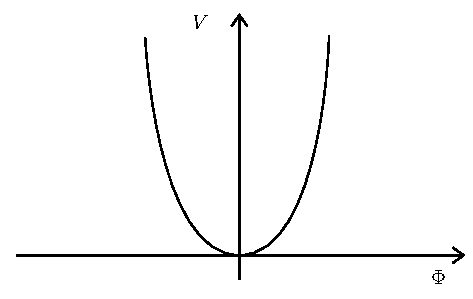
\includegraphics[width=0.6\textwidth]{../lessons/n_image/1.pdf}
\caption{\label{fig:} Description.}
\end{figure}

  \item Case \( T<T_c \) \( (r_0<0) \): there are two solutions \( \Phi _0 = \pm \sqrt{-\frac{r_0}{u_0}}  \).
  \begin{figure}[h!]
  \centering
  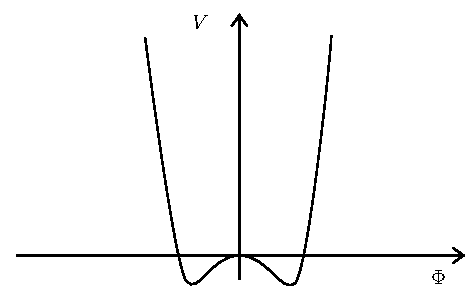
\includegraphics[width=0.6\textwidth]{../lessons/n_image/2.pdf}
  \caption{\label{fig:} Description.}
  \end{figure}

\end{enumerate}
\begin{remark}
The two solution \( \pm \Phi _0 \) are related by the transformation \( \in \mathbb{Z}^2 \): \( \Phi \rightarrow - \Phi  \).
\end{remark}
\begin{remark}
For \( T < T_c \) the two states (phases) \( \pm \Phi _0 \) have a lower symmetry than the state \( \Phi _0 = 0 \).
\end{remark}
\begin{remark}
If the thermal fluctuations \( \delta \Phi  \) are sufficiently strong to allow passages between the two states \( \pm \Phi _0 \) at \( T < T_c \), we have \( \expval{\Phi } = 0  \) (preserves states).
\end{remark}
However, for \( T < T_c \) and \( N \rightarrow + \infty  \), transition between the two states will be less and less probable and the system will be trapped into one of the two states \( (\pm \Phi _0) \). The system choose spontaneously one of the two less symmetric state. Therefore, its physics is not any more described by \( \Phi  \) but the fluctuations \( \delta \Phi  \) around the chosen minimum \( \Phi _0 \). There is spontaneous symmetry breaking.

The variable \( \Phi  \) is not any more symmetric and one has to look at \( \Phi \rightarrow \Phi _0 + \delta \Phi  \), where \( \delta \Phi  \) is a new variable!


\section{Spontaneous breaking of continuous symmetries and the anset of Goldstone particles}
Let us start with a simple model in which the order parameter is a scalar complex variable
\begin{equation}
  \Phi = \frac{\Phi _1 + i \Phi _2}{\sqrt{2} }
\end{equation}
and with an \( \mathcal{H} \) that is invariant with respect to a global continuous transformation.

The simplest model in statistical mechanics is the XY model with \( O(2) \) symmetry or a GL model for a superfluid or superconductor (no magnetic field)
\begin{equation}
  \mathcal{H}_{eff} = \int_{}^{} \dd[D]{\va{x}} \qty[\grad \Phi \vdot \grad \Phi ^* + \frac{r_0}{2} \Phi ^* \Phi + \frac{u_0}{4} \qty(\Phi ^* \Phi )^2 ]
\end{equation}
where
\begin{equation}
  \Phi (\va{x}) = \frac{1}{\sqrt{2} } \qty[ \Phi _1 (\va{x}) + i \Phi _2 (\va{x})]
\end{equation}
or
\begin{equation}
  \Phi (\va{x}) = \psi (\va{x}) e^{i \alpha (\va{x})}
\end{equation}
\begin{itemize}
\item Superfluid: \( \Phi  \) macroscopic wave function of the Bose condensate (density of superfluid \( n= \abs{\Phi ^2}  \)).
\item Superconductor: \( \Phi  \) single particle wave function describing the position of the centre of mass of the Cooper pair.
\end{itemize}

\subsection{Quantum relativistic case (field theory)}
The analog of \( \mathcal{H} \) is the action
\begin{equation}
  S(\Phi ) = \int_{}^{} \dd[D]{\va{x}}   \mathcal{L} ( \Phi )
\end{equation}
where
\begin{equation}
  \mathcal{L} (\Phi ) = - \frac{1}{2} \partial_\mu \Phi \partial^\mu \Phi ^*
  - \frac{r_0}{2} \Phi \Phi ^* - \frac{u_0}{4} \qty(\Phi \Phi ^*)^2
\end{equation}
It describes a scalar complex (i.e. charged) muonic field with mass \( m \). Note that in this case \( r_0>0 \) and \( m \equiv \sqrt{r_0}  \). The term \( (\Phi \Phi ^*)^2 \) means self-interaction with strenght \( \lambda \equiv u_0 \).

In all cases, the original symmetry is \( U(1) \), i.e. both \( \mathcal{H} \) and \( \mathcal{L} \) are invariant with respect to the transformation
\begin{equation}
  \Phi \rightarrow e^{i \theta } \Phi , \quad \Phi ^* \rightarrow e^{-i \theta } \Phi ^*
  \label{eq:n_1}
\end{equation}
\begin{remark}
The phase \( \theta  \) does not depend on \( \va{x} \) (global symmetry).
\end{remark}
In components \eqref{eq:n_1} become
\begin{equation}
  \begin{cases}
   \Phi _1 \rightarrow  \Phi _1 \cos \theta - \Phi _2 \sin \theta \\
  \Phi _2 \rightarrow  \Phi _2 \cos \theta + \Phi _1 \sin \theta
  \end{cases}
\end{equation}
\begin{equation}
  (\Phi _1', \Phi _2') = \begin{pmatrix}
  \cos \theta    & - \sin \theta   \\
    \sin \theta  & \cos \theta
  \end{pmatrix}
  \begin{pmatrix}
  \Phi _1 \\
  \Phi _2
  \end{pmatrix}
\end{equation}
Let us focus first on the statistical mechanics model and to the most interesting case of \( r_0 <0 \).

In components \( \mathcal{H} \) becomes
\begin{equation}
  \mathcal{H} = \int_{}^{} \dd[D]{\va{x}} \qty[\qty(\grad \Phi _1)^2 + \qty(\grad \Phi _2)^2  ] + \int_{}^{} \dd[D]{\va{x}} V (\Phi _1, \Phi _2)
\end{equation}
where
\begin{equation}
  V (\Phi _1, \Phi _2) = \frac{r_0}{2} \qty(\Phi _1^2 + \Phi _2^2) + \frac{u_0}{4} \qty( \Phi _1^2 + \Phi _2^2)^2
\end{equation}
It is the mexican hat potential, shown in Figure \ref{fig:n_1}

\begin{figure}[h!]
\centering
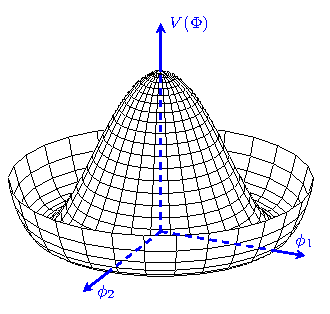
\includegraphics[width=0.6\textwidth]{../lessons/n_image/3.pdf}
\caption{\label{fig:n_1} Case \( r_0 < 0 \).}
\end{figure}

For \( r_0 < 0 \), there is a uniform solution \( (\grad \Phi _1 = \grad \Phi _2 = 0) \). Let \( S = \sqrt{\Phi _1^2 + \Phi _2^2}  \),
\begin{equation}
  V (S) = \frac{r_0}{2} S^2 + \frac{u_0}{4} S^4
\end{equation}
\begin{equation}
  \dv{V(S)}{S} = r_0 S + u_0 S^3 = 0
\end{equation}
There is 1 maximum at \( S=0 \) and minima for \( S^2 = - \frac{r_0}{u_0} \)

For \( r_0 < 0 \), \( \mathcal{H} \) displays minima when
\begin{equation}
  \Phi _1^2 + \Phi _2^2 \equiv v^2 = - \frac{r_0}{u_0}
\end{equation}
On the \( 2D \) plane \( (\Phi _1, \Phi _2) \) the minima lie on the circle of radius
\begin{equation}
  v = \sqrt{- \frac{r_0}{u_0}}
\end{equation}
The spontaneous symmetry breaking occurs when the system "chooses" one of the infinite available minima.

In our example, suppose that the chosen minimum is
\begin{equation}
  \Phi _1 = v = \sqrt{- \frac{r_0}{u_0}}, \quad \Phi _2 = 0
\end{equation}
\begin{figure}[h!]
\centering
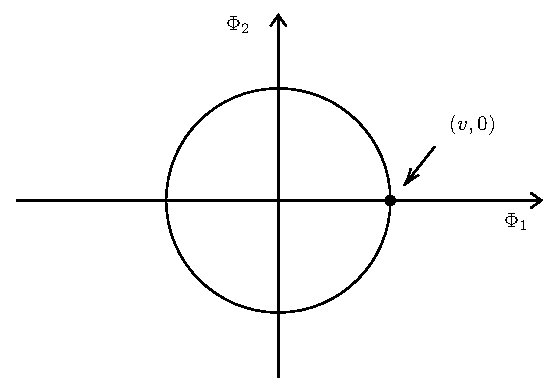
\includegraphics[width=0.6\textwidth]{../lessons/n_image/4.pdf}
\caption{\label{fig:n_4} Description.}
\end{figure}

\section{Interpretation in relativistic quantum mechanics}
\begin{enumerate}
\item \( r_0 <0 \) corresponds to an imaginary mass. This is because to move away from \( \Phi =0 \), the system experiences a negative resistence in both directions, being \( \Phi =0 \) a relative local minimum.

\item The minimum has the lowest energy and therefore it must correspond to the empty state.
In this case, however, there is an infinite number of empty states!
\end{enumerate}
Summarizing: the starting Hamiltonian (or Lagrangian) is invariant with respect to \( U(1) \) but the one that describes the fluctuation dynamics around one of the chosen minimum state is not invariant with respect to \( U(1) \).

Let us now write the Lagrangian with respect to the fluctuations of \( \Phi _1  \)  and \( \Phi _2 \) around the chosen state
\begin{equation}
  \begin{cases}
   \Phi _1 = v + \delta \Phi _1\\
   \Phi _2 = 0 + \delta \Phi _2
  \end{cases}
\end{equation}
or
\begin{equation}
  \Phi = v + \qty(\delta \Phi _1 + i \delta \Phi _2)
\end{equation}
Note that, since
\begin{equation}
  \begin{cases}
   \delta \Phi _1 = \Phi _1 - v\\
   \delta \Phi _2 = \Phi _2
  \end{cases}
\end{equation}
we have
\begin{equation}
  \expval{\delta \Phi _1} _{\Phi _0 } = \expval{\delta \Phi _2}_{\Phi _0} = 0
\end{equation}
As expected the expectation of the empty state is back to be zero.

For the quantum relativistic Lagrangian, let us write
\begin{equation}
  r_0 \rightarrow m^2, \quad u_0 \rightarrow \lambda , \quad v^2 = - \frac{m^2}{\lambda }
\end{equation}

\begin{equation}
\begin{split}
\mathcal{L}  = & - \frac{1}{2} \partial _ \mu \qty(\delta \Phi _1 + i \delta \Phi _2)   \partial _ \mu \qty(\delta \Phi _1 - i \delta \Phi _2)  \\
 & - \frac{m^2}{2} \qty(v + \delta \Phi _1 + i \delta \Phi _2) \qty(v + \delta \Phi _1 - i \delta \Phi _2) \\
 & - \frac{\lambda }{4} \qty[ \qty(v + \delta \Phi _1 + i \delta \Phi _2) \qty(v + \delta \Phi _1 - i \delta \Phi _2) ] ^2 \\
 =& - \frac{1}{2} \qty(\partial_ \mu  \delta \Phi _1 \partial^ \mu \delta \Phi _1  )
 - \frac{1}{2} \qty( \partial_ \mu  \delta \Phi _2 \partial^\mu \delta \Phi _2  )  \\
 & - \frac{m^2}{2} \qty(v^2 + 2 v \delta \Phi _1 + \delta \Phi _1^2 + \delta \Phi _2^2) \\
 &- \frac{\lambda }{4} \qty(v^2 + 2 v \delta \Phi _1 + \delta \Phi _1^2 + \delta \Phi _2 ^2)^2
\end{split}
\end{equation}
Since \( m^2 = - v^2 \lambda  \),
\begin{equation}
\begin{split}
\mathcal{L}   = &  - \frac{1}{2} \qty(\partial_ \mu  \delta \Phi _1 \partial^ \mu \delta \Phi _1  )
- \frac{1}{2} \qty( \partial_ \mu  \delta \Phi _2 \partial^ \mu \delta \Phi _2  ) \\
& + \frac{\lambda v^2}{2} \qty(v^2 + 2 v \delta \Phi _1 + \delta \Phi _1^2 + \delta \Phi _2^2)  \\
& - \frac{\lambda }{4} \qty(v^4 + 4 v^2 \delta \Phi _1^2 + \qty(\delta \Phi _1^2 + \delta \Phi _2^2)^2
    4 v^3 \delta \Phi _1 + 2 v^2 \qty(\delta \Phi _1^2 + \delta \Phi _2^2) + 4 v \delta \Phi _1 \qty(\delta \Phi _1^2 + \delta \Phi _2^2)   )
\end{split}
\end{equation}
Neglecting the constant terms in \( v \)
\begin{equation}
\begin{split}
\mathcal{L} \qty(\delta \Phi _1, \delta \Phi _2)   = &  - \frac{1}{2} \qty(\partial_ \mu  \delta \Phi _1 )^2 - \frac{1}{2} \qty(\partial_ \mu \delta \Phi _2 )^2    \\
& - \lambda v^2 \delta \Phi _1^2 - v \lambda \delta \Phi _1 \qty( \qty(\delta \Phi _1)^2 + \qty(\delta \Phi _2 )^2  ) \\
& - \frac{\lambda }{4} \qty( \qty(\delta \Phi _1)^2 + \qty(\delta \Phi _2)^2  )^2
\end{split}
\end{equation}
\begin{remark}
The term \( - \lambda v^2 \delta \Phi _1^2 \) indicates that the field \( \delta \Phi _1 \) (related to the transversal fluctuations) has a null empty state \( ( \expval{\delta \Phi _1}= 0 ) \) and a mass \( M \) such that:
\begin{equation}
  M^2 = 2 \lambda v^2 = - 2 r_0
\end{equation}
Therefore, it represents a real, massive, mesonic scalar field that is physically accettable.

However, \( \mathcal{L} \) is not any more invariant under the transformation \( \delta \Phi _1 \rightarrow - \delta \Phi _1 \).
\end{remark}
\begin{remark}
The field \( \delta \Phi _2 \) has no mass! It describes the fluctuations along the circle where the potential \( V \) is in its minimum  which imples no dynamical inertia, that implies no mass!
\end{remark}
So, starting with one complex scalar field \( \Phi (\va{x}) \) having mass \( m \), when \( m^2 < 0 \)one gets a real scalar field \( \delta \Phi _1 \) with mass \( M = \sqrt{- 2 m^2}  \)  and a second scalar field \( \delta \Phi _2 \) that is massless. This is called the \emph{Goldstone boson}.
\begin{theorem}[]
If a continuous symmetry is spontaneously broken and there are no long range interactions, exists an elementary eccitation with zero momentum or particle of zero mass called Goldstone boson.
\end{theorem}
More generally, let \( \mathcal{P} \) be a subgroup of \( \mathcal{G} \). If \( \mathcal{G} \) has \( N \) indipendent generators and \( \mathcal{P} \)  has \( M \) indipendent generators, if \( \mathcal{P} \) is the new (lower) symmetry, therefore exist \( N-M \)  Goldstone bosons.

In the previous case \( \mathcal{G} = U (1)  \Rightarrow  N=1\) whereas \( M=0 \) (we have chosen a specific minimum).
\begin{example}
XY model in statistical mechanics:
\begin{itemize}
\item \( \delta \Phi _1 \): fluctuation of the modulus of \( m \).
\item \( \delta \Phi _2 \): fluctuations of the spin directions \( \Rightarrow  \) spin waves.
\end{itemize}
\end{example}
\begin{remark}
In particle physics the presence of Goldstone bosons brings a serious problem in field theory since the corresponding particles are not observed!
\end{remark}

\subsubsection{Higgs-Englert-Brout (1964)}
Higgs mechanism gives back the mass to the Goldstone particles.
The basic idea is that the Goldstone theorem that works for a continuous global symmetry it can fail for loacl gauge theories!

\section{Spontaneous symmetry breaking in Gauge symmetries}
Statistical mechanics, Gl model for superconductors in presence of a magnetic field (\emph{Meissner effect}, i.e. the magnetic induction \( \va{B} = 0 \) inside the superconductor).

\begin{equation}
  \mathcal{H} (\Phi ) = \int_{}^{} \dd[D]{\va{x}} \qty[\frac{1}{2}B^2 + \abs{\qty(\va{\grad }- 2 i \va{A})\Phi  }^2 ] + \frac{r_0}{2} \Phi ^* \Phi
  + \frac{u_0}{4} \qty(\Phi ^* \Phi )^2 - \va{B} \vdot \va{H}
\end{equation}
where \( \frac{B^2}{2} \) is the energy of the magnetic field \( \va{B} \) and \( \va{\grad } \rightarrow \qty[\va{\grad } + i q \va{A}]  \) is the minimal coupling.
Consider \( \va{H} \) the external magnetic field
\begin{equation}
  \va{B} = \va{H} + \va{M}
\end{equation}
is the induction field.

Normal conductor corresponding to \( \Phi _0 = 0 \), that implies \( \va{B} = \va{H} \). For a superconfuctor we have \( \Phi \neq 0 \), a spontaneous symmetry breaking.   



\end{document}
